
\documentclass[12pt]{article}
\usepackage{float}
%\usepackage[bottom]{footmisc}
\usepackage{cite}
\usepackage{graphicx}
\usepackage{algorithm}
\usepackage{algorithmic}
\usepackage{longtable}
\usepackage{color}
\usepackage[section]{placeins}
\usepackage{hyperref}
\hypersetup{
colorlinks=true,
    linkcolor=blue,
    urlcolor=red,
    linktoc=all
}
\graphicspath{{figures/}} % Graphics will be here

%
% Pagestyle
%
\oddsidemargin9.6mm
\evensidemargin9.6mm
\topmargin-1cm
\headheight20pt
\textwidth155mm
\textheight232mm
\pagestyle{myheadings}
%
% Macros
%
\newcommand\fbe{{\tt fbe\_tez}}
\newcommand\report{{\tt report}}
\newcommand{\bq}{\begin{quotation}\noindent}
\newcommand{\eq}{\end{quotation}}
\renewcommand{\arg}[1]{$\langle\mbox{\it #1}\rangle$}
%
% Title declarations
%

\title{{\Huge CmpE 443 Final Project Design Document} \\ Group Name: Tezla  }
\author{Members \\ Abdurrahman DILMAC (Team Leader) \\ Ahmet Semih ARI\\ Ramazan ARSLAN\\ Yunus Emre DEMIRCI}


\date{December 29, 2018 \\ Version 2.00}

\begin{document}
\maketitle

\newpage
\tableofcontents
\newpage

%
% Block Diagram
%


\section{System Level Structural Diagram (Block Diagram)} % pending 
\label{sec:block}


\begin{figure}[htbp]
\begin{center}
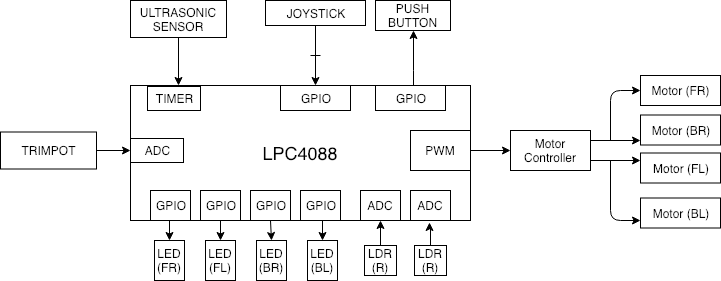
\includegraphics[width=1\columnwidth]{figures/443-Diagram-block.png}
\end{center}
\caption{Block Diagram of car.}
\vskip\baselineskip % Leave a vertical skip below the figure
\label{fig:sample}
\end{figure}

\textbf{LPC4088 Microcontroller:} Main part of the car. Runs software and controls peripherals.

\textbf{Motor controller:} By getting inputs from the main board, controls motors by means of controlling speed, directions, soft and hard brakes.

\textbf{Motor:} Gives tork to the car, and thus moves.

\textbf{LEDs:} Emits light, controlled by the main board. Used for car signals.

\textbf{Joystick:} Takes input from the player/user and informs the main board, so it can take appropriate action.


\textbf{Push Button:} It is used to toggle mode to Manuel and Auto with interrupts. 

\textbf{Ultrasonic sensor:} Car can measure distance with ultrasonic sensor. 

\textbf{Trimpot:} Used to adjust motor speed. It can take value between 0-100. 


\newpage


\section{System Level Functional Diagram}
\begin{figure}[htbp]
\begin{center}
\hspace*{-1.1in}
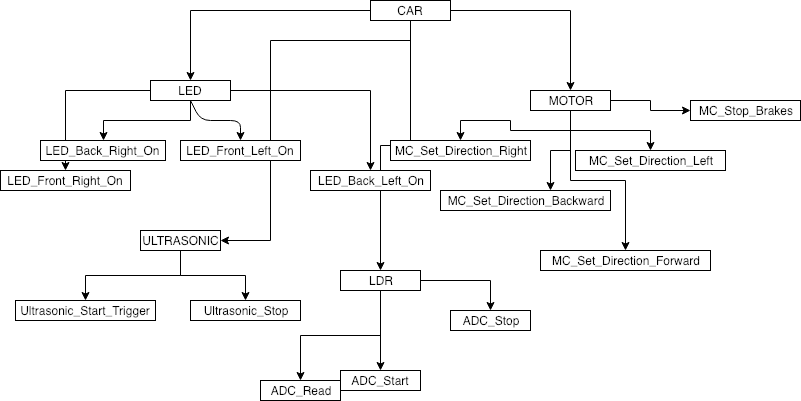
\includegraphics[width=1.30\columnwidth]{func.png}
\end{center}
\caption{System Level Functional Diagram}
\vskip\baselineskip % Leave a vertical skip below the figure
\label{fig:sample}
\end{figure}

\newpage

\section{Sequence Diagrams} % pending 

\subsection{Manual Mode}
\FloatBarrier
\begin{figure}[htbp]
\begin{center}
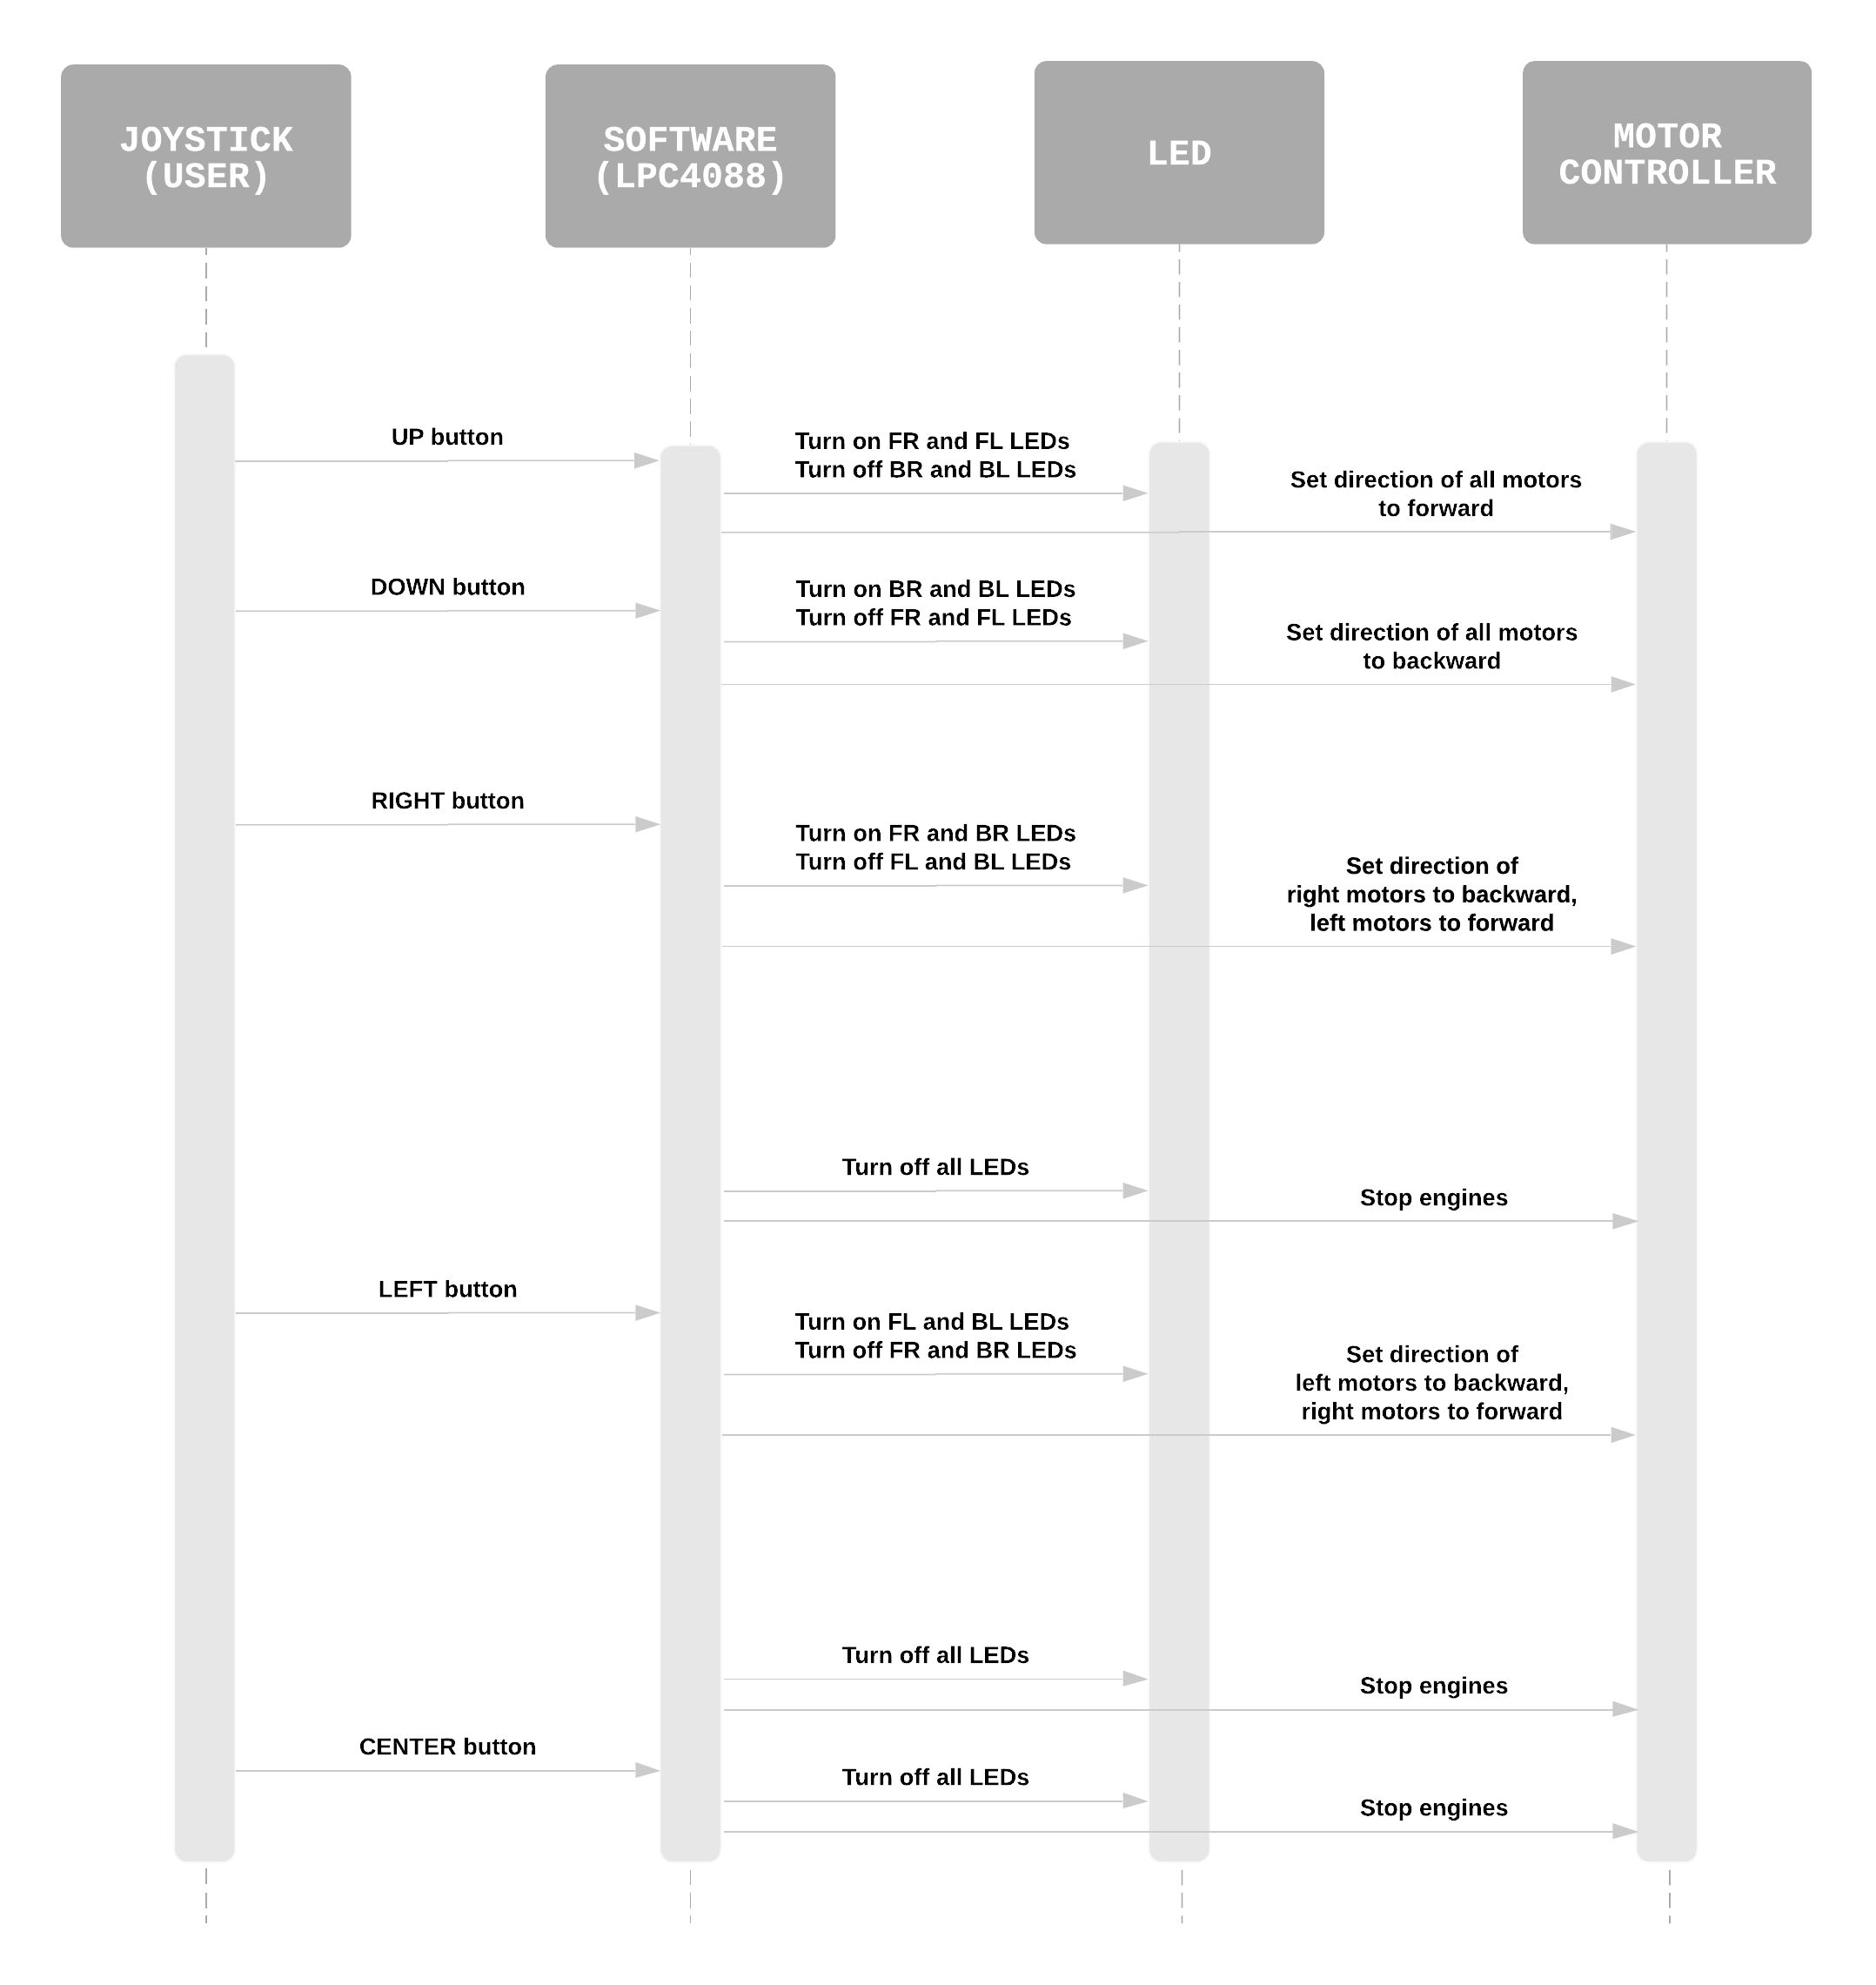
\includegraphics[width=1\columnwidth]{figures/sequence-diagram1.png}
\end{center}
\caption{Sequence Diagram of Manual Mode.}
\label{fig:sample}
\end{figure}

\newpage

\subsection{Autonomous Mode}

\begin{figure}[htbp]
\begin{center}
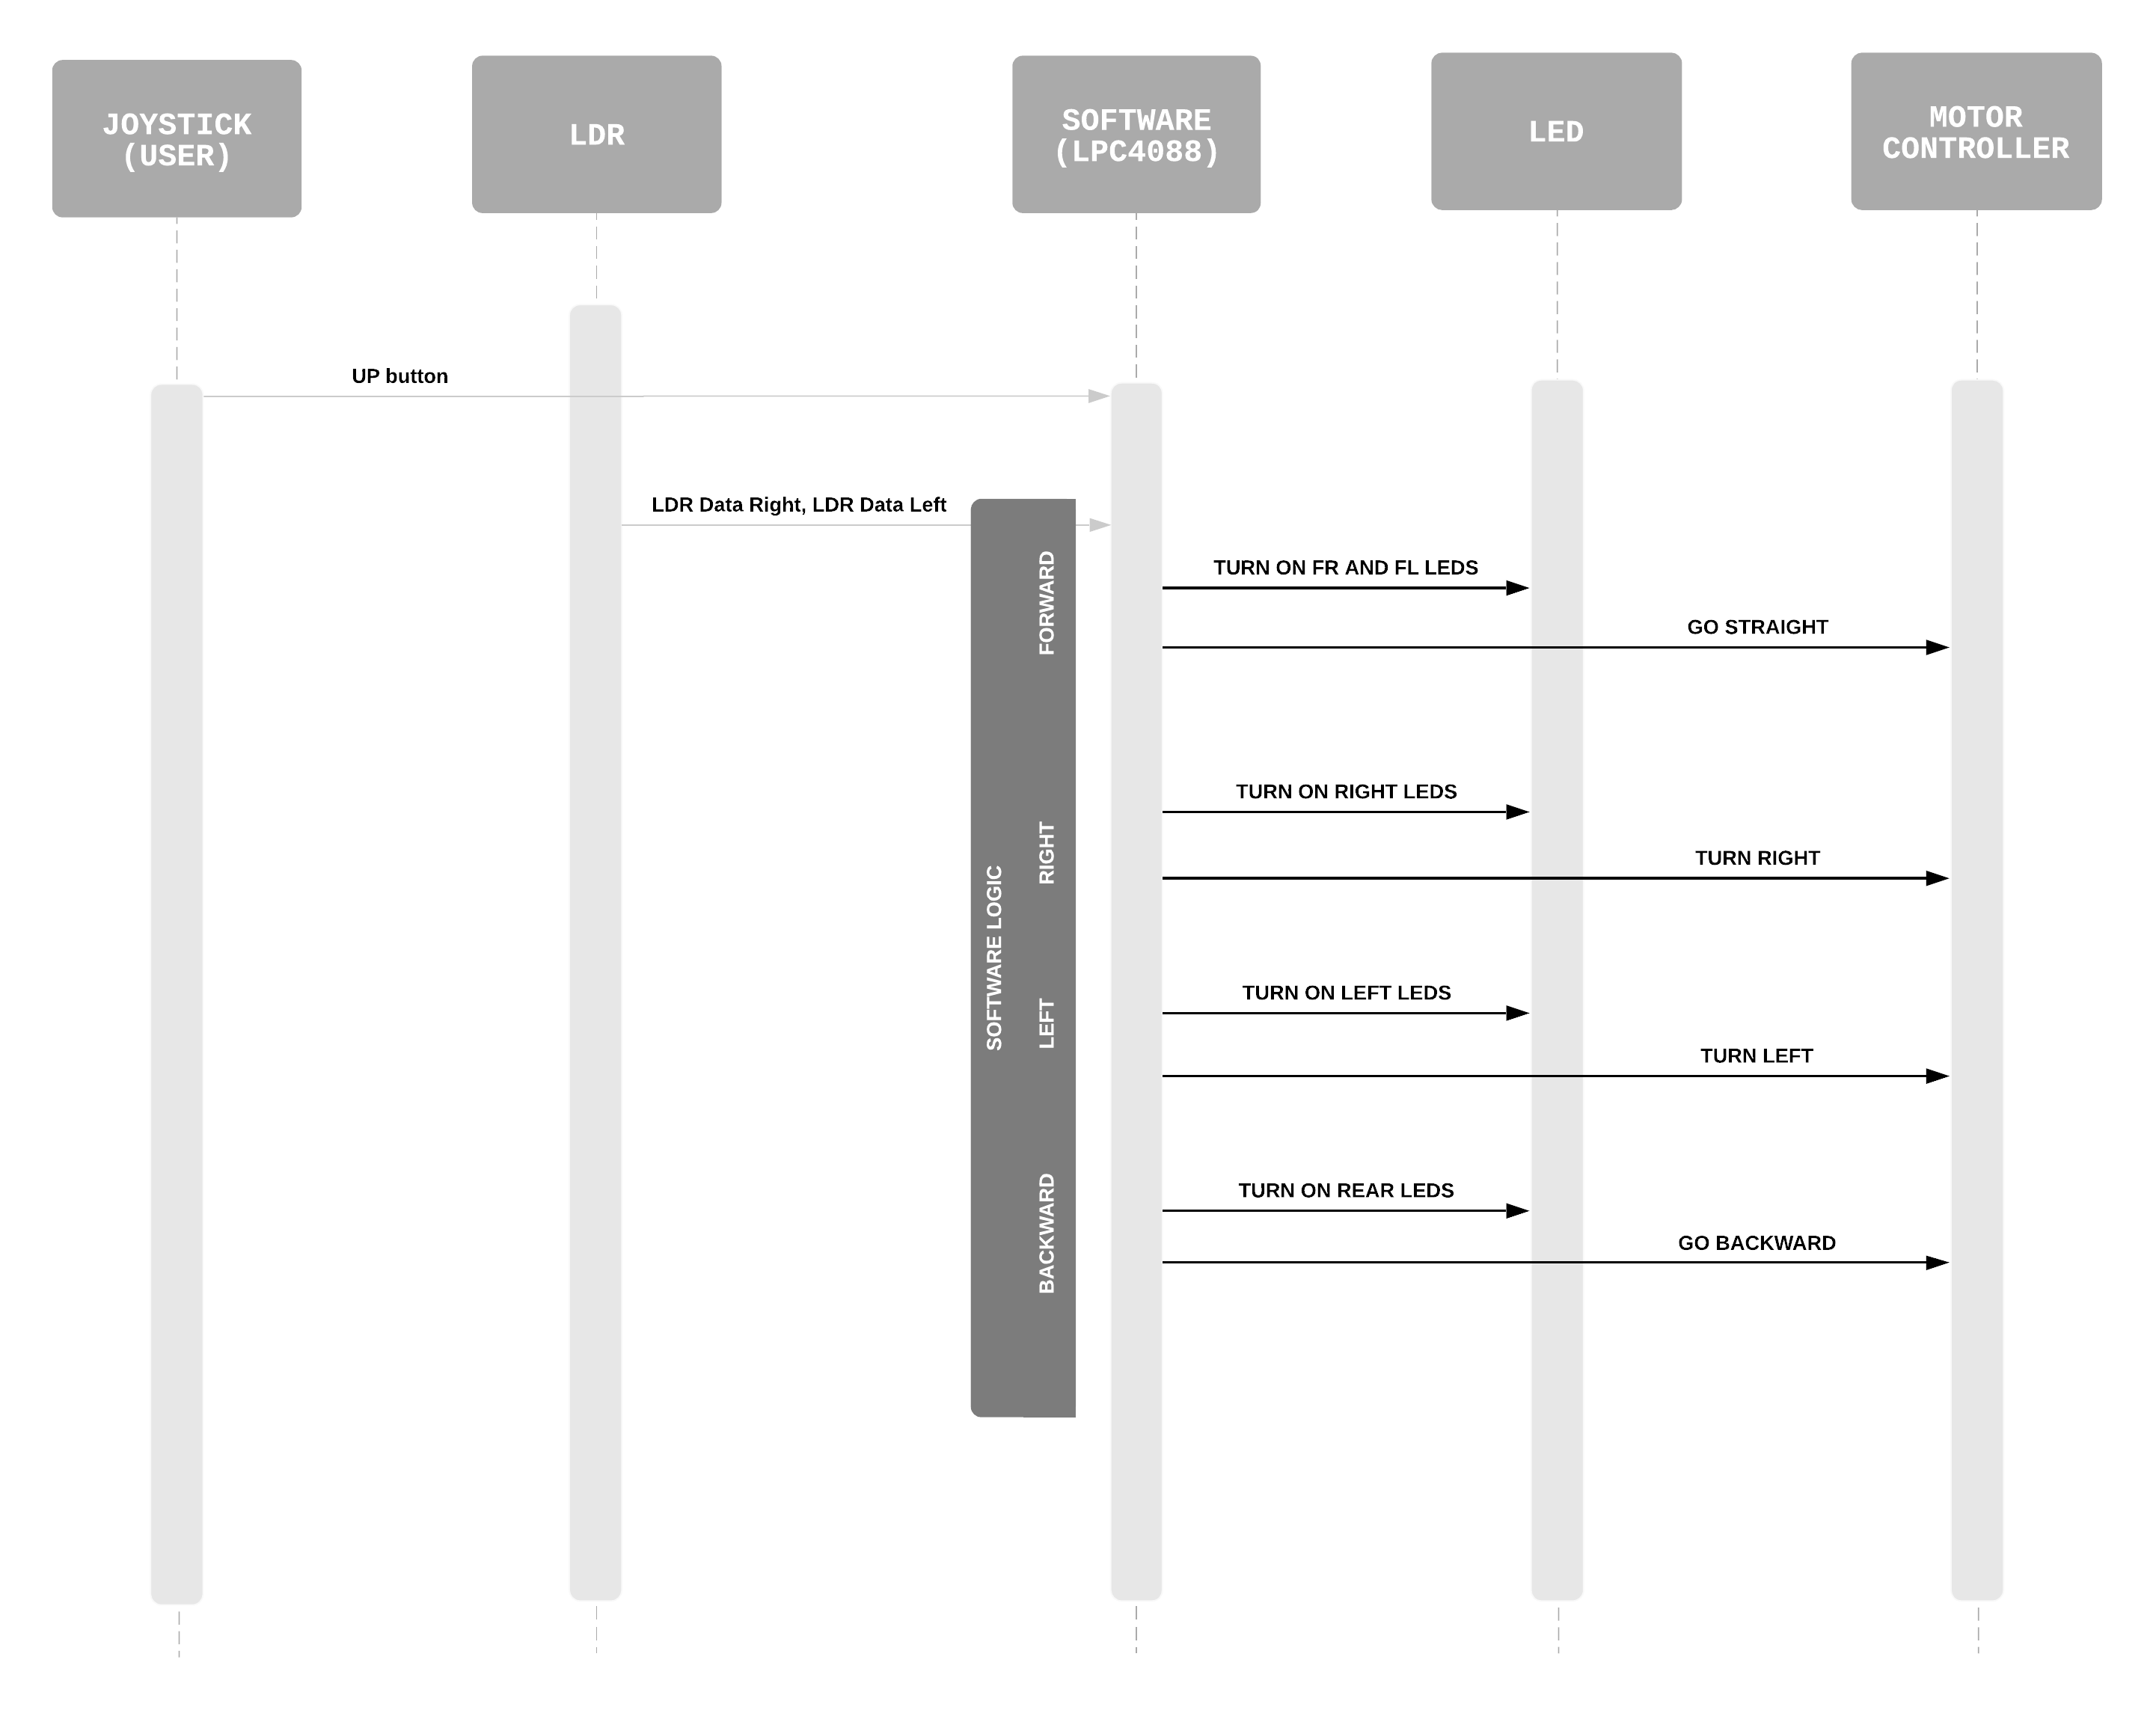
\includegraphics[width=1\columnwidth]{figures/sequence-diagram2.png}
\end{center}
\caption{Sequence Diagram of Autonomous Mode.}
\label{fig:sample}

\end{figure}


\newpage



\section{Connections} % pending 

\subsection{LED Connections}
All the components which are controlled via LPC4088 should be connected to the board. Therefore, you should determine the pins and their functionalities. Draw the described table in the term project interim report description document. After you determine the all the pins, draw the circuit schematic for the LED circuits. \\

\begin{center}
\begin {table}[H]
\begin{tabular}{|c|c|c|c|c|}
\hline
The LED name & LPC4088 PIN & Port & Pin Functionality & Reason \\\hline
Front Right LED & PIN5 & P1.24 & GPIO & Supports digital I/O \\\hline
Front Left LED & PIN6 & P1.23 & GPIO & Supports digital I/O \\\hline
Back Right LED & PIN7 & P1.20 & GPIO & Supports digital I/O \\\hline
Back Left LED & PIN8 & P0.21 & GPIO & Supports digital I/O \\\hline
\end{tabular}
\caption{LED Pins and their functionalities}
\end{table}
\end{center}


\subsection{LDR Connections}

\begin {table}[H]
\begin{center}
\begin{tabular}{|c|c|c|c|c|}
\hline
Motor driver PIN & LPC4088 PIN & Port & Pin Functionality & Reason \\\hline
GND & PIN1 & GND & Ground & Common ground \\\hline
LDR left  & PIN17 & PORT0\_25 & ADC0\_IN[2] & Convert digital\\\hline
LDR right & PIN18 & PORT0\_26 & ADC0\_IN[3] & Convert digital \\\hline
VCC & PIN45 & Vout & Power input & 3.3V needed \\\hline
\end{tabular}
\caption{Ultrasonic Sensor and Board PIN connections with their functionalities.}
\end{center}
\end{table}

\subsection{Motor - Motor Controller Connections}

There is only one motor controller to control 4 motors. Output A is used for right motors and Output B is for left motors.

\begin {table}[H]
\begin{center}
\begin{tabular}{|c|c|}
\hline
Motor Terminal & Motor Driver Terminal \\\hline
Motor 1 + & Output A + \\\hline
Motor 1 - & Output A - \\\hline
Motor 2 + & Output A + \\\hline
Motor 2 - & Output A - \\\hline
Motor 3 + & Output B + \\\hline
Motor 3 - & Output B - \\\hline
Motor 4 + & Output B + \\\hline
Motor 4 - & Output B - \\\hline
\end{tabular}
\caption{Motor Controller and Motor connections.}
\end{center}
\end{table}


\subsection{Motor Controller - Board Connections}

Here is the table depicting relations between the board and motor controller:

\begin {table}[H]
\begin{center}
\begin{tabular}{|c|c|c|c|c|}
\hline
Motor driver PIN & LPC4088 PIN & Port & Pin Functionality & Reason \\\hline
Power GND & PIN1 & GND & Ground & Ground is needed \\\hline
+5V Power & PIN44 & Vout & Power input & For transferring voltage \\\hline
A Enable & PIN29 & P1.3 & PWM0\_1 (ENA) & Supports PWM Output \\\hline
B Enable & PIN30 & P1.2 & PWM0\_2 (ENB) & Supports PWM Output \\\hline
IN1 & PIN12 & P0.8 & GPIO & Supports digital I/O \\\hline
IN2 & PIN13 & P0.7 & GPIO & Supports digital I/O \\\hline
IN3 & PIN9 & P0.0 & GPIO & Supports digital I/O \\\hline
IN4 & PIN10 & P0.1 & GPIO & Supports digital I/O \\\hline
\end{tabular}
\caption{Motor Controller and Board PIN connections with their functionalities.}
\end{center}
\end{table}


\subsection{Ultrasonic Connections}

Here is the table depicting relations between the board and ultrasonic sensor:

\begin {table}[H]
\begin{center}
\begin{tabular}{|c|c|c|c|c|}
\hline
Motor driver PIN & LPC4088 PIN & Port & Pin Functionality & Reason \\\hline
GND & PIN1 & GND & Ground & Common ground \\\hline
Trigger & PIN11 & P0.9 & T2\_MAT\_3 & Send Trigger with Timer2\\\hline
Echo & PIN16 & P0.24 & T3\_CAP\_1 & Capture Echo with Timer3 \\\hline
VCC & PIN44 & Vout & Power input & 5V needed \\\hline
\end{tabular}
\caption{Ultrasonic Sensor and Board PIN connections with their functionalities.}
\end{center}
\end{table}



\newpage



\section{Circuit Schematics} % pending 
\label{sec:schematics}

\subsection{LED Circuit Schematics}

\begin{figure}[!htb]
\begin{center}
%\hspace*{-1in}
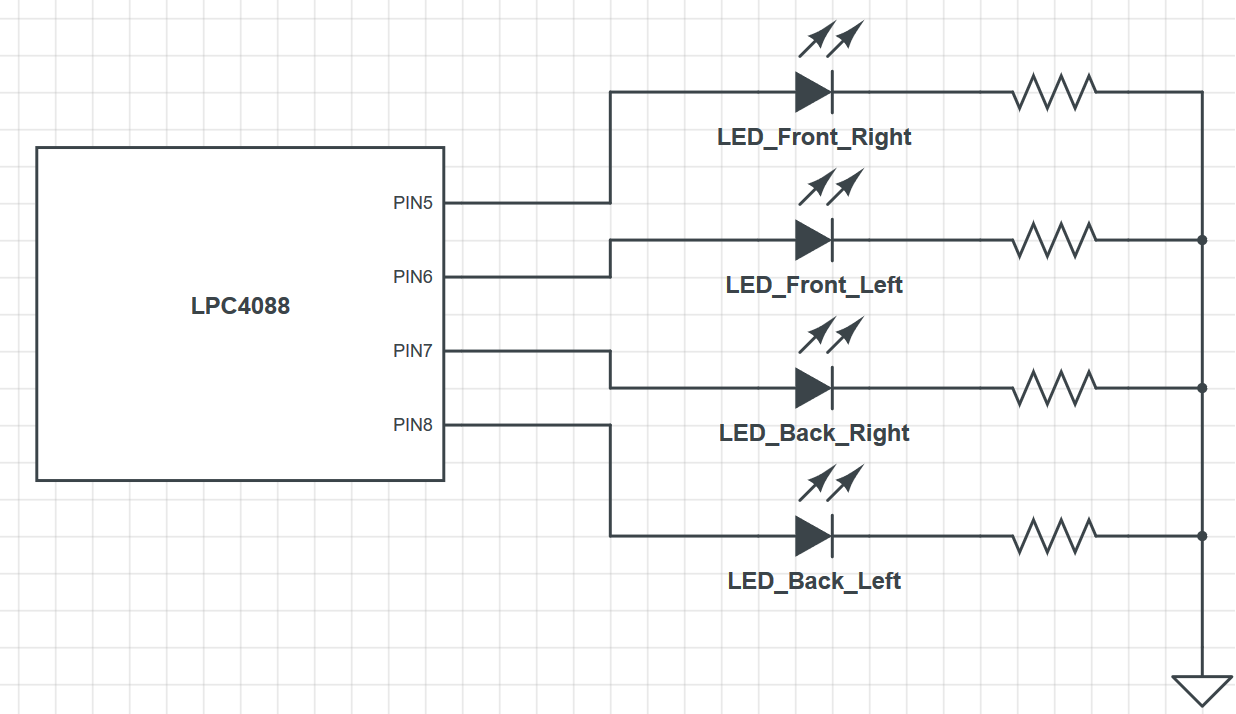
\includegraphics[width=1\columnwidth]{led-circuit-diagram.png}
\end{center}
\caption{LED Circuit Diagram.}
\vskip\baselineskip % Leave a vertical skip below the figure
\label{fig:led}
\end{figure}
\FloatBarrier

\newpage
\subsection{LDR Circuit Schematics}
\label{sec:ldrschema}

\begin{figure}[!htb]
\begin{center}
%\hspace*{-1in}
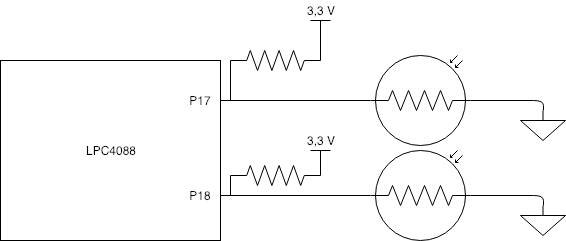
\includegraphics[width=1\columnwidth]{figures/LDR.png}
\end{center}
\caption{LDR Circuit Diagram.}
\vskip\baselineskip % Leave a vertical skip below the figure
\label{fig:ldr}
\end{figure}
\FloatBarrier

\subsection{Motor - Motor Controller Circuit Schematics}
\begin{figure}[!htb]
\begin{center}
%\hspace*{-1in}
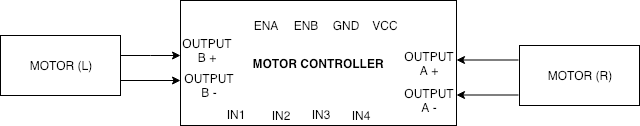
\includegraphics[width=1\columnwidth]{figures/motor-motorcontrol.png}
\end{center}
\caption{Motor - Motor Controller Circuit Diagram.}
\vskip\baselineskip % Leave a vertical skip below the figure
\label{fig:sample}
\end{figure}
\FloatBarrier

\newpage
\subsection{Motor Controller - Board Circuit Schematics}
\begin{figure}[!htb]
\begin{center}
%\hspace*{-1in}
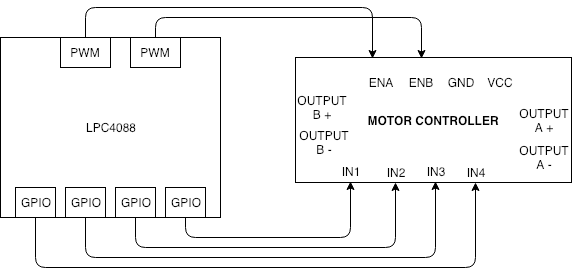
\includegraphics[width=1\columnwidth]{figures/motorcontrol-board.png}
\end{center}
\caption{Motor Controller - Board Circuit Diagram.}
\vskip\baselineskip % Leave a vertical skip below the figure
\label{fig:sample}
\end{figure}
\FloatBarrier


\newpage



\section{Expense List} % done 
There are not much expense.

\begin{table}[H]
    \centering
    \begin{tabular}{|c|c|}
        \hline
        Name & Expense \\\hline
        Cables & 5 TRY \\\hline
        Document Printing & 3 TRY \\\hline
    \end{tabular}
    \caption{Expenses}
    %\label{tab:my_label}
\end{table}
\newpage



\section{Pseudocodes}

\begin{algorithm}
\caption{init}
\begin{algorithmic} 
\STATE	Initilaze LED
\STATE	Initilaze PWM
\STATE	Initilaze Joystick
\STATE	Initilaze Timer
\STATE	Initilaze ADC
\STATE	Initilaze UART
\STATE	Initilaze UARTInterrupt
\STATE	Initilaze MotorController
\STATE	Initilaze UltrasonicTriggerTimer
\STATE	Initilaze UltrasonicCaptureTimer
\STATE	Initilaze ExternalInterrupt
\end{algorithmic}
\end{algorithm}

\begin{algorithm}
\caption{Manuel}
\begin{algorithmic} 
\IF{Forward Flag}
\IF{ ultrasonicSensorDistance $<$ obstacleDistance}
\STATE isApproachedTo15 $\leftarrow$ true
\STATE Set Backward Flag and Motor and Led	
\ENDIF
\IF{leftLDR $<$ Treshold}
\STATE Set Right Motor and Led
\ELSIF{rightLDR $<$ Treshold}
\STATE Set Left Motor and Led
\ELSE
\STATE Set Forward Motor and Led
\ENDIF
\ENDIF
\IF{isApproachedTo15 and ultrasonicSensorDistance $>$ escapeDistance}
\STATE isApproachedTo15 $\leftarrow$ false
\STATE Set Forward Flag and Motor and Led
\ENDIF

\IF{Joystick Up Pressed}
\STATE Set Forward Flag and Motor and Led
\ELSIF{Joystick Right Pressed}
\STATE Set Right Flag and Motor and Led
\ELSIF{Joystick Left Pressed}
\STATE Set Left Flag and Motor and Led
\ELSIF{Joystick Down Pressed}
\STATE Set Backward Flag and Motor and Led
\ELSIF{Joystick Center Pressed}
\STATE Set Stop Flag and Motor and Led
\ENDIF
\IF{Right Flag}
\IF{TIMER3$\rightarrow$TC mod SECOND $<$ SECOND / 2}
\STATE RightLED
\ELSE
\STATE OffLED
\ENDIF
\ENDIF
\IF{Left Flag}
\IF{TIMER3$\rightarrow$TC mod SECOND $<$ SECOND / 2}
\STATE LeftLED
\ELSE
\STATE OffLED
\ENDIF
\ENDIF
\end{algorithmic}
\end{algorithm}

\begin{algorithm}
\caption{Auto}
\begin{algorithmic}
\IF{Joystick Up Pressed or autoDirection $>$ 0}
\STATE autoDirection $\leftarrow$ Forward

\IF{(leftLDR $>$ actLDR and RightLDR $>$ actLDR) or LDRDataLeft$-$LDRDataRight $<$ toleranceLDR
or LDRDataRight$-$LDRDataLeft $<$ toleranceLDR}
\STATE Set Forward Flag and Motor and Led
\STATE inflateLeft $\leftarrow$ 0
\STATE inflateRight $\rightarrow$ 0
\ELSIF{LDRDataLeft $<$ actLDR and LDRDataRight $>$ actLDR} 
\STATE Set Right Flag and Motor and Led
\STATE autoDirection $\leftarrow$ Right
\STATE inflateRight
\ELSIF{LDRDataRight $<$ actLDR and LDRDataLeft $>$ actLDR} 
\STATE Set Left Flag and Motor and Led
\STATE autoDirection $\leftarrow$ Left
\STATE inflateLeft
\ENDIF

\IF{inflateRight $>$ 500 or inflateLeft $>$ 500}
\STATE $inflatedSpeed \leftarrow TrimpotDataValue/2$
\ELSE 
\STATE $inflatedSpeed \leftarrow TrimpotDataValue$
\ENDIF

\STATE RightMotorSpeed $\leftarrow$ inflatedSpeed
\STATE LeftMotorSpeed $\leftarrow$ inflatedSpeed



\IF{ ultrasonicSensorDistance $<$ obstacleDistance}
\STATE isApproachedTo15 $\leftarrow$ true
\STATE Set Backward Flag and Motor and Led	
\ENDIF
\IF{isApproachedTo15 and ultrasonicSensorDistance $>$ escapeDistance}
\STATE isApproachedTo15 $\leftarrow$ false
\STATE Set Forward Flag and Motor and Led
\ENDIF
\IF{autoDirection is Right}
\IF{TIMER3$\rightarrow$TC mod SECOND $<$ SECOND / 2}
\STATE RightLED
\ELSE
\STATE OffLED
\ENDIF
\ENDIF
\IF{autoDirection is Left}
\IF{TIMER3$\rightarrow$TC mod SECOND $<$ SECOND / 2}
\STATE LeftLED
\ELSE
\STATE OffLED
\ENDIF
\ENDIF
\ENDIF
\end{algorithmic}
\end{algorithm}

\begin{algorithm}
\caption{update}
\begin{algorithmic} 
\REQUIRE TrimpotValue,  DriveMode and autoDirection from Interrupt, leftLDR, rightLDR
\STATE StartUltrasonicTrigger
\STATE RightMotorSpeed $\leftarrow$ TrimpotValue
\STATE LeftMotorSpeed $\leftarrow$ TrimpotValue
\IF{DriveMode is Manuel}
\STATE Manuel
\ELSE
\STATE Auto
\ENDIF
\end{algorithmic}
\end{algorithm}



\begin{algorithm}
\caption{main}
\begin{algorithmic} 
\STATE init
\WHILE{$ 1 $}
\STATE update
\ENDWHILE
\end{algorithmic}
\end{algorithm}

\end{document}
%
% End of fbeman.tex